% Options for packages loaded elsewhere
\PassOptionsToPackage{unicode}{hyperref}
\PassOptionsToPackage{hyphens}{url}
\PassOptionsToPackage{dvipsnames,svgnames,x11names}{xcolor}
%
\documentclass[
  super,
  preprint,
  3p]{elsarticle}

\usepackage{amsmath,amssymb}
\usepackage{lmodern}
\usepackage{iftex}
\ifPDFTeX
  \usepackage[T1]{fontenc}
  \usepackage[utf8]{inputenc}
  \usepackage{textcomp} % provide euro and other symbols
\else % if luatex or xetex
  \usepackage{unicode-math}
  \defaultfontfeatures{Scale=MatchLowercase}
  \defaultfontfeatures[\rmfamily]{Ligatures=TeX,Scale=1}
\fi
% Use upquote if available, for straight quotes in verbatim environments
\IfFileExists{upquote.sty}{\usepackage{upquote}}{}
\IfFileExists{microtype.sty}{% use microtype if available
  \usepackage[]{microtype}
  \UseMicrotypeSet[protrusion]{basicmath} % disable protrusion for tt fonts
}{}
\makeatletter
\@ifundefined{KOMAClassName}{% if non-KOMA class
  \IfFileExists{parskip.sty}{%
    \usepackage{parskip}
  }{% else
    \setlength{\parindent}{0pt}
    \setlength{\parskip}{6pt plus 2pt minus 1pt}}
}{% if KOMA class
  \KOMAoptions{parskip=half}}
\makeatother
\usepackage{xcolor}
\setlength{\emergencystretch}{3em} % prevent overfull lines
\setcounter{secnumdepth}{5}
% Make \paragraph and \subparagraph free-standing
\ifx\paragraph\undefined\else
  \let\oldparagraph\paragraph
  \renewcommand{\paragraph}[1]{\oldparagraph{#1}\mbox{}}
\fi
\ifx\subparagraph\undefined\else
  \let\oldsubparagraph\subparagraph
  \renewcommand{\subparagraph}[1]{\oldsubparagraph{#1}\mbox{}}
\fi


\providecommand{\tightlist}{%
  \setlength{\itemsep}{0pt}\setlength{\parskip}{0pt}}\usepackage{longtable,booktabs,array}
\usepackage{calc} % for calculating minipage widths
% Correct order of tables after \paragraph or \subparagraph
\usepackage{etoolbox}
\makeatletter
\patchcmd\longtable{\par}{\if@noskipsec\mbox{}\fi\par}{}{}
\makeatother
% Allow footnotes in longtable head/foot
\IfFileExists{footnotehyper.sty}{\usepackage{footnotehyper}}{\usepackage{footnote}}
\makesavenoteenv{longtable}
\usepackage{graphicx}
\makeatletter
\def\maxwidth{\ifdim\Gin@nat@width>\linewidth\linewidth\else\Gin@nat@width\fi}
\def\maxheight{\ifdim\Gin@nat@height>\textheight\textheight\else\Gin@nat@height\fi}
\makeatother
% Scale images if necessary, so that they will not overflow the page
% margins by default, and it is still possible to overwrite the defaults
% using explicit options in \includegraphics[width, height, ...]{}
\setkeys{Gin}{width=\maxwidth,height=\maxheight,keepaspectratio}
% Set default figure placement to htbp
\makeatletter
\def\fps@figure{htbp}
\makeatother

\usepackage{amsmath}
\usepackage{booktabs}
\usepackage{caption}
\usepackage{longtable}
\makeatletter
\makeatother
\makeatletter
\makeatother
\makeatletter
\@ifpackageloaded{caption}{}{\usepackage{caption}}
\AtBeginDocument{%
\ifdefined\contentsname
  \renewcommand*\contentsname{Table of contents}
\else
  \newcommand\contentsname{Table of contents}
\fi
\ifdefined\listfigurename
  \renewcommand*\listfigurename{List of Figures}
\else
  \newcommand\listfigurename{List of Figures}
\fi
\ifdefined\listtablename
  \renewcommand*\listtablename{List of Tables}
\else
  \newcommand\listtablename{List of Tables}
\fi
\ifdefined\figurename
  \renewcommand*\figurename{Figure}
\else
  \newcommand\figurename{Figure}
\fi
\ifdefined\tablename
  \renewcommand*\tablename{Table}
\else
  \newcommand\tablename{Table}
\fi
}
\@ifpackageloaded{float}{}{\usepackage{float}}
\floatstyle{ruled}
\@ifundefined{c@chapter}{\newfloat{codelisting}{h}{lop}}{\newfloat{codelisting}{h}{lop}[chapter]}
\floatname{codelisting}{Listing}
\newcommand*\listoflistings{\listof{codelisting}{List of Listings}}
\makeatother
\makeatletter
\@ifpackageloaded{caption}{}{\usepackage{caption}}
\@ifpackageloaded{subcaption}{}{\usepackage{subcaption}}
\makeatother
\makeatletter
\@ifpackageloaded{tcolorbox}{}{\usepackage[many]{tcolorbox}}
\makeatother
\makeatletter
\@ifundefined{shadecolor}{\definecolor{shadecolor}{rgb}{.97, .97, .97}}
\makeatother
\makeatletter
\makeatother
\journal{To be determined}
\ifLuaTeX
  \usepackage{selnolig}  % disable illegal ligatures
\fi
\usepackage[]{natbib}
\bibliographystyle{elsarticle-num}
\IfFileExists{bookmark.sty}{\usepackage{bookmark}}{\usepackage{hyperref}}
\IfFileExists{xurl.sty}{\usepackage{xurl}}{} % add URL line breaks if available
\urlstyle{same} % disable monospaced font for URLs
\hypersetup{
  pdftitle={A Bayesian Perspective},
  pdfauthor={James M Brophy MD PhD},
  pdfkeywords={extracorporeal CPR, Bayesian statistics},
  colorlinks=true,
  linkcolor={blue},
  filecolor={Maroon},
  citecolor={Blue},
  urlcolor={Blue},
  pdfcreator={LaTeX via pandoc}}

\setlength{\parindent}{6pt}
\begin{document}

\begin{frontmatter}
\title{A Bayesian Perspective \\\large{Extracorporeal CPR for Refractory
Out-of-Hospital Cardiac Arrest} }
\author[1]{James M Brophy MD PhD%
\corref{cor1}%
\fnref{fn1}}
 \ead{james.brophy@mcgill.ca} 

\affiliation[1]{organization={McGill University Health Center, Centre
for Health Outcomes Research (CORE)},addressline={5252 Boul. de
Maisonneuve West Room 2B.37},city={Montreal},postcode={H4A
3S5},postcodesep={}}

\cortext[cor1]{Corresponding author}
\fntext[fn1]{JMB is a research scholar supported by Les Fonds de
Recherche Québec Santé}
        
\begin{abstract}
A recent randomized clinical trial, INCEPTION, reported in patients with
refractory out-of-hospital cardiac arrest, extracorporeal CPR (eCPR) and
conventional CPR (cCPR) had similar effects on survival with a favorable
neurologic outcome. The current study examines if a Bayesian perspective
provides additional insights. Depending on the prior selected, the
Bayesian approach for the INCEPTION intention-to treat (ITT) analysis
shows an equivalence probability between 13.4 - 16.8\% (defined as 1 /
1.1 \textless{} odds ratio (OR) \textless{} 1.1). The probability of
clinical superiority with eCPR ranges from 65.7 - 77.0 \% (defined as OR
\textgreater{} 1.1). A similar analyses using INCEPTION per protocol
(PP) data shows an equivalence probability between 4.7 - 20.2\% with
reduced probabilities of clinical superiority not exceeding 25\%. It is
concluded that a Bayesian perspective allows considerable additional
insights into the trial analysis and interpretation. The non-negligible
probabilities of increased survival with their considerable residual
uncertainties, suggests that additional studies are required before
concluding that eCPR and cCPR have similar survival effects.
\end{abstract}





\begin{keyword}
    extracorporeal CPR \sep 
    Bayesian statistics
\end{keyword}
\end{frontmatter}
    \ifdefined\Shaded\renewenvironment{Shaded}{\begin{tcolorbox}[breakable, sharp corners, enhanced, interior hidden, boxrule=0pt, borderline west={3pt}{0pt}{shadecolor}, frame hidden]}{\end{tcolorbox}}\fi

\hypertarget{introduction}{%
\section{Introduction}\label{introduction}}

Out-of-hospital cardiac arrest is a frequent event and fortunately its
devastating consequences can be partially mitigated by rapid
commencement of basic life support with high-quality chest compressions
and external defibrillation (conventional cardiopulmonary resuscitation
(cCPR)). However, there remains a substantial subset of individuals who
do not respond rapidly to these measures and whether more invasive
measures. Whether the addition of more aggressive measure including
extracorporeal CPR (the addition of extracorporeal membrane oxygenation
to standard advanced cardiac life support (eCPR)) can improve survival
and diminish anoxic brain injury is a current topic of research. A large
randomized clinical trial (RCT) examining this question recently
published their results\citep{CPR2023a}. For their primary outcome, 30
day survival without significant neurological deficit, an odds ratio of
1.4 (95\% confidence interval, 0.5 to 3.5; P = 0.52) in favor of
extracorporeal CPR was observed leading to the conclusion ``In patients
with refractory out-of-hospital cardiac arrest, extracorporeal CPR and
conventional CPR had similar effects on survival with a favorable
neurological outcome''.\citep{CPR2023a}

This communication does not reiterate the many reasons to be wary of
null hypothesis significance testing (NHST), p values and confidence
intervals\citep{RN5420}. Rather it assumes the reader has perhaps heard
that Bayesian methods mirror our intuitive learning and diagnostic
processes and is curious about its potential application to RCT analyses
and interpretations.

Therefore the goal of this communication is to examine whether a
Bayesian perspective permits additional insights into the specific
clinical question regarding any added value of eCPR following an
out-of-hospital arrest in patients refractory to cCPR.

\hypertarget{methods}{%
\section{Methods}\label{methods}}

The data for the primary outcome, 30 day survival with intact
neurological status, based on an intention to treat (ITT) analysis was
abstracted from the original INCEPTION trial \citep{CPR2023a} and used
for the primary analysis. The ITT analysis has the advantage of
minimizing bias by preserving the prognostic balance afforded by
randomization as well as assuring the validity of the accompanying
statistical analyses.

Bayesian analytical approaches provide a number of benefits over the
classical NHST approach, including parameter estimation accompanied by
direct probability statements about parameters of interest (herein the
risk of survival with intact neurological status), and the incorporation
prior knowledge \citep{BrophyCardio, Zampieri}.

These probability statements arise from the posterior distribution
according to the Bayes Thereom, expressed as follows:
\[ \text{Posterior}  = \frac{\text{Probability of the data} * \text{Prior}}{\text{Normalizing Constant}} \]

Therefore, in addition to the current data summarized by the probability
of the data (likelihood function), prior probability distributions are
required. Because our main focus is the analysis and interpretation of
the INCEPTION trial alone, our primary analysis used a default vague
parameter prior (\(log(\theta) \sim Normal [0, 2.50]\), thereby assuring
that the posterior distribution is dominated by the observed INCEPTION
data.

The robustness of the Bayesian approach is often assessed by sensitivity
analyses that examine the variation in the posterior probability as a
function of the choice of different prior distributions. Incorporating
prior information underscores another important advantage of Bayesian
analyses, the ability to learn sequentially. There were two previous
RCTs examining extracorporeal CPR\citep{RN6759, RN6751} and while the
protocols are not identical, it may be reasonable to allow this data to
serve as informed priors for the eCPR parameter, which can be updated
with the INCEPTION data.

Therefore, in addition to the vague prior described above, we considered
three possible informative priors\\
i) a \textbf{combined} prior using all the available prior RCT
data\citep{RN6751, RN6759}\\
ii) an \textbf{enthusiastic} prior, so labelled since this uses only the
ARREST data, a trial stopped prematurely for efficacy\\
iii) a \textbf{skeptical} prior, so labelled since this uses only the
PRAGUE data, a trial stopped prematurely for futility

This prior information of the probability of eCPR success in each
previous trial, \(X_i\), can be summarized as a normal distribution with
a mean equal to the proportion of successes, \(\hat{p_i}\) with a
standard deviation equal to \[\sqrt{\hat{p_i}*(1-\hat{p_i})}\] As
baseline success rates for cCPR varies markedly between the three
studies, it was decided to maintain the INCEPTION control baseline with
the vague prior for all analyses and to update only the eCPR arm with
prior information.

Posterior distributions are summarized with medians and 95\%
highest-density intervals (credible intervals (CrI)), defined as the
narrowest interval containing 95\% of the probability density function
\citep{mcelreath2020}. Bayesian analyses permit not only calculations of
the posterior probability of any additional survival with eCPR (OR
\textgreater1.00), but also of clinically meaningful benefits. While
there is no universal definition for a clinically meaningful benefit, a
survival OR \textgreater1.10 may be an acceptable threshold for many.
Bayesian analyses also allows calculation of the probability between any
two points. For example, rather than simply comparing if the survival of
one treatment is better than another, one can calculate a range of
practical equivalence (ROPE) between treatments. While different ranges
may be proposed, +/- 10\% seems a reasonable small difference that many
woul consider as equivalent.

ITT assesses subjects based on the group they were initially (and
randomly) allocated to, regardless of whether or not they dropped out,
were fully adhered to the treatment or switched to an alternative
treatment. In superiority trials, ITT analyses can therefore be seen as
a conservative estimate which mirrors clinical effectiveness. In
contrast, a per protocol (PP) analysis accounts for adherence by
analyzing only those patients who completed the treatment they were
originally allocated to. While PP may provide additional insights into
efficacy, it is subject to bias. Since a PP analysis when performed in
conjunction with an ITT analysis may provide additional insights, this
has also been subjected to a Bayesian analysis.

Posterior distributions were estimated using the Hamiltonian Monte
Carlo,a form of Markov Chain Monte Carlo simulations in which the
gradient of the log posterior is used to efficiently sample the
posterior space. This was implemented in \texttt{Stan}\citep{stan} using
the front end \texttt{rstanarm} package\citep{rstanarm} by fitting a
logistic regression model with a single treatment parameter. All
analyses were executed using \texttt{R}\citep{R} within the integrated
development environmentof RStudio\citep{Rstudio}. The statistical code
can be found on Github (https://github.com/brophyj/eCPR).

\hypertarget{results}{%
\section{Results}\label{results}}

ITT data from the INCEPTION trial\citep{CPR2023a} and two other
pertinent trials\citep{RN6759, RN6751} that also randomized out of
hospital cardiac arrest patients to cCPR to eCPR are shown in Table 1.
Performing a Bayesian analysis on the INCEPTION trial, using a default
vague prior, produces an odds ratio (OR) 1.32 with 95\% CrI 0.54 - 3.22.
The closeness of this result to the original analysis (OR, 1.4; 95\% CI
0.5 - 3.5) confirms the minimal impact of the default vague prior and
reveals a Bayesian analysis completely dominated by the observed
INCEPTION data.

One of the advantages of a Bayesian approach is the ability to make
direct probability statements about the estimand of improved eCPR
survival. The eCPR probability density function for improved survival
from INCEPTION data with the default vague prior is displayed in Figure
1 and reveals that the probability of enhanced survival with eCPR is
72.7\%. The probability that the improved survival exceeds a 10\%
improvement is 65.7\% and the ROPE probability is 13.4\% (Table 2).

Three different informative priors were considered i) a N(0.32, 0.47)
ii) a N(0.43, 0.49) iii) a N(0.31, 0.46) distributions to represent all
the combined available RCT data\citep{RN6759, RN6751}, only the
ARREST\citep{RN6751} data and only the PRAGUE\citep{RN6759} data,
respectively

These different prior probabilities were updated using with the
INCEPTION ITT data to create the posterior distributions displayed in
Table 2. The probability for enhanced eCPR survival has increased to
80.4\% with a skeptical prior to 84.9\% with the enthusiastic prior and,
as expected, the associated uncertainty has been reduced, as reflected
by the narrower 95\% CrI, with the additional data. The posterior
probability of improved eCPR survival goes from 80\% with a skeptical
prior to 85\% with the enthusiastic prior. The probability that the eCPR
survival improvements exceed the proposed 10\% clinical threshold are
71\% and 77\% for the skeptical and enthusiastic priors, respectively.
The corresponding ROPE probabilities are 16.8\% and 13.8\% (Table 2).
Posterior probabilities with the combined prior fell as expected between
the results with the skeptical and enthusiastic priors. The graphical
presentations of these results are shown in Figure 2.

INCEPTION did not report a per-protocol analysis. Such an analysis may
be helpful in assessing treatment efficacy, unfortunately at the risk of
an increased risk of bias by not respecting the ITT principle. From
INCEPTION Figure S4\citep{CPR2023a}, it appears that the per protocol
data for mortality is 13 survivors from 61 patients in the cCPR group
compared to 5 survivors from 46 patients receiving eCPR. With a vague
prior, the OR of increased survival with eCPR is decreased compared to
cCPR but with very wide CrI (OR 0.45, 95\% CrI 0.15 - 1.35), limiting
any definitive conclusions. The decreased eCPR success rates in the
INCEPTION PP data results in reduced posterior probabilities of eCPR
benefit and an increased probability of equivalence or benefit with
cCPR. The exact probabilities of increased eCPR survival incorporating
the previous identified informative priors are shown in Table 3.

\hypertarget{discussion}{%
\section{Discussion}\label{discussion}}

This Bayesian analysis of the INCEPTION ITT data alone (with a vague
prior) suggests the presence of a non-negligible probability of benefit
with eCPR, in the range of 73\%, compared to cCPR. The probability that
this improvement in survival exceeds 10\% is almost 66\%. The
consideration of pertinent prior information from two previous
RCTs\citep{RN6751, RN6759} in the field results in estimates of improved
eCPR survival probabilities, with intact neurological status, in the
vicinity of 80-85\%. Moreover depending on the choice of prior beliefs
included, the posterior probability of at least a 10\% improved eCPR
survival is in the range of 71 - 77\% probability. In contrast to the
INCEPTION original conclusion of similar survival effects between the
two treatment, this re-analysis suggests only a modest probability of
approximately that survival probabilities between the two techniques are
within a reasonably acceptable equivalence range. The overall message
would appear to be that while any definitive conclusions regarding the
superiority of eCPR are lacking, the possibility of a clinically
meaningful benefit or even less likley clinically meaningful harm has
not been reasonably excluded and continued research is necessary to
clarifying the remaining uncertainties.

The INCEPTION researchers are to be congratulated on their trial design,
its execution, and addressing an important clinical question in the most
challenging of research environments. However the natural constraints of
standard statistical analyses, also known as null hypothesis
significance testing, limits the full exploitation of the current data
and updating of past knowledge. For trails failing to meet statistical
significance, those incorrectly labelled ``negative'' trials, null
hypothesis significance testing favors confusion ``between absence of
evidence and evidence of absence''\citep{RN6765}.

\newpage

\hypertarget{tables}{%
\section{Tables}\label{tables}}

\setlength{\LTpost}{0mm}
\begin{longtable}{lcccc}
\caption*{
{\large Table 1 Extracted ITT trial data}
} \\ 
\toprule
Trial & Fail CPR (n) & Fail eCPR (n) & Success CPR (n) & Success eCPR (n) \\ 
\midrule
INCEPTION & 52 & 56 & 10 & 14 \\ 
ARREST & 15 & 8 & 0 & 6 \\ 
PRAGUE & 108 & 86 & 24 & 38 \\ 
\bottomrule
\end{longtable}
\begin{minipage}{\linewidth}
eCPR = extracorporeal cardiopulmonary resuscitation\\
\end{minipage}

\setlength{\LTpost}{0mm}
\begin{longtable}{lcccccc}
\caption*{
{\large Table 2 eCPR odds ratios, 95\% credible intervals and probabilities with various priors}
} \\ 
\toprule
Priors & OR & \multicolumn{2}{c}{95\% CrI} & \multicolumn{3}{c}{Probabilities} \\ 
\cmidrule(lr){1-1} \cmidrule(lr){2-2} \cmidrule(lr){3-4} \cmidrule(lr){5-7}
 & point estimate & lower limit & upper limit & p(OR) >1  & p(OR) >1.1  &  p(ROPE) \\ 
\midrule
Vague & $1.321$ & $0.543$ & $3.215$ & 0.727 & $0.657$ & 0.134 \\ 
Combined & $1.349$ & $0.705$ & $2.580$ & 0.817 & $0.732$ & 0.153 \\ 
Enthusiastic & $1.403$ & $0.738$ & $2.668$ & 0.849 & $0.770$ & 0.138 \\ 
Skeptical & $1.322$ & $0.700$ & $2.496$ & 0.804 & $0.710$ & 0.168 \\ 
\bottomrule
\end{longtable}
\begin{minipage}{\linewidth}
Vague: default vague prior\\
Combined: prior eCPR data from ARREST + PRAGUE\\
Enthusiastic: prior eCPR data from ARREST alone\\
Skeptical: prior eCPR data from PRAGUE alone\\
ROPE: range of practical equivalence = + / - 10\% OR (odds ratio)\\
\end{minipage}

\setlength{\LTpost}{0mm}
\begin{longtable}{lcccccc}
\caption*{
{\large Table 3 eCPR (per protocol) odds ratios, 95\% credible intervals and probabilities with various priors}
} \\ 
\toprule
Priors & OR & \multicolumn{2}{c}{95\% CrI} & \multicolumn{3}{c}{Probabilities} \\ 
\cmidrule(lr){1-1} \cmidrule(lr){2-2} \cmidrule(lr){3-4} \cmidrule(lr){5-7}
 & point estimate & lower limit & upper limit & p(OR) >1  & p(OR) >1.1  &  p(ROPE) \\ 
\midrule
Vague & $0.451$ & $0.151$ & $1.348$ & $0.070$ & $0.049$ & $0.047$ \\ 
Combined & $0.859$ & $0.430$ & $1.713$ & $0.330$ & $0.238$ & $0.202$ \\ 
Enthusiastic & $0.870$ & $0.437$ & $1.734$ & $0.345$ & $0.251$ & $0.201$ \\ 
Skeptical & $0.858$ & $0.419$ & $1.755$ & $0.327$ & $0.237$ & $0.197$ \\ 
\bottomrule
\end{longtable}
\begin{minipage}{\linewidth}
Vague: default vague prior\\
Combined: prior eCPR data from ARREST + PRAGUE\\
Enthusiastic: prior eCPR data from ARREST alone\\
Skeptical: prior eCPR data from PRAGUE alone\\
ROPE: range of practical equivalence = + / - 10\% OR (odds ratio)\\
\end{minipage}

\newpage

\hypertarget{figures}{%
\section{Figures}\label{figures}}

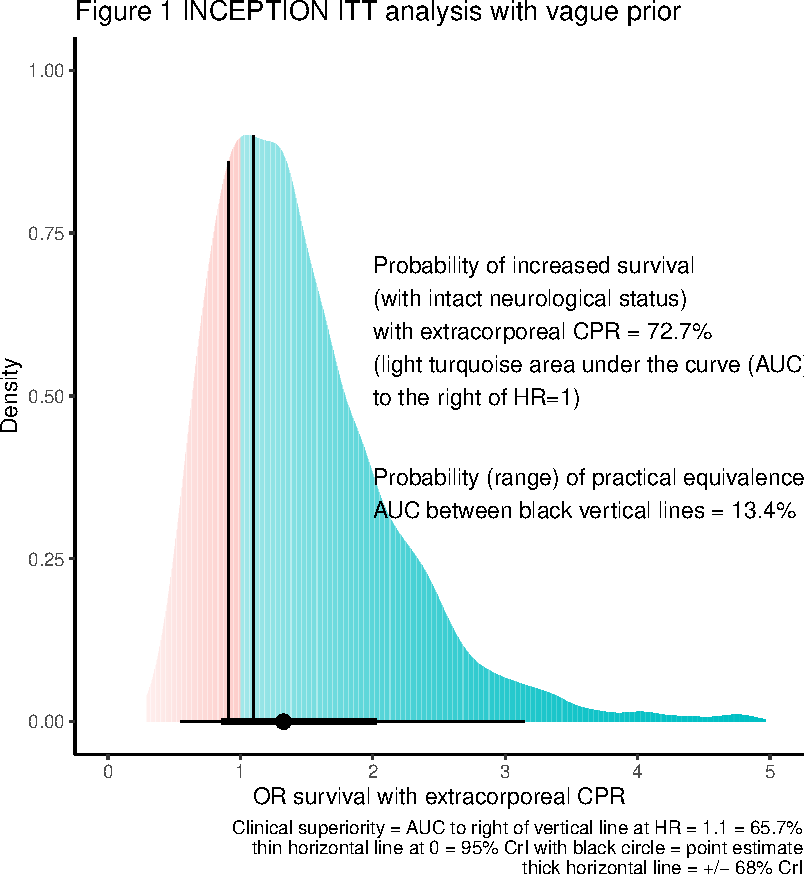
\includegraphics{manuscript_files/figure-pdf/fig1-1.pdf}

\newpage

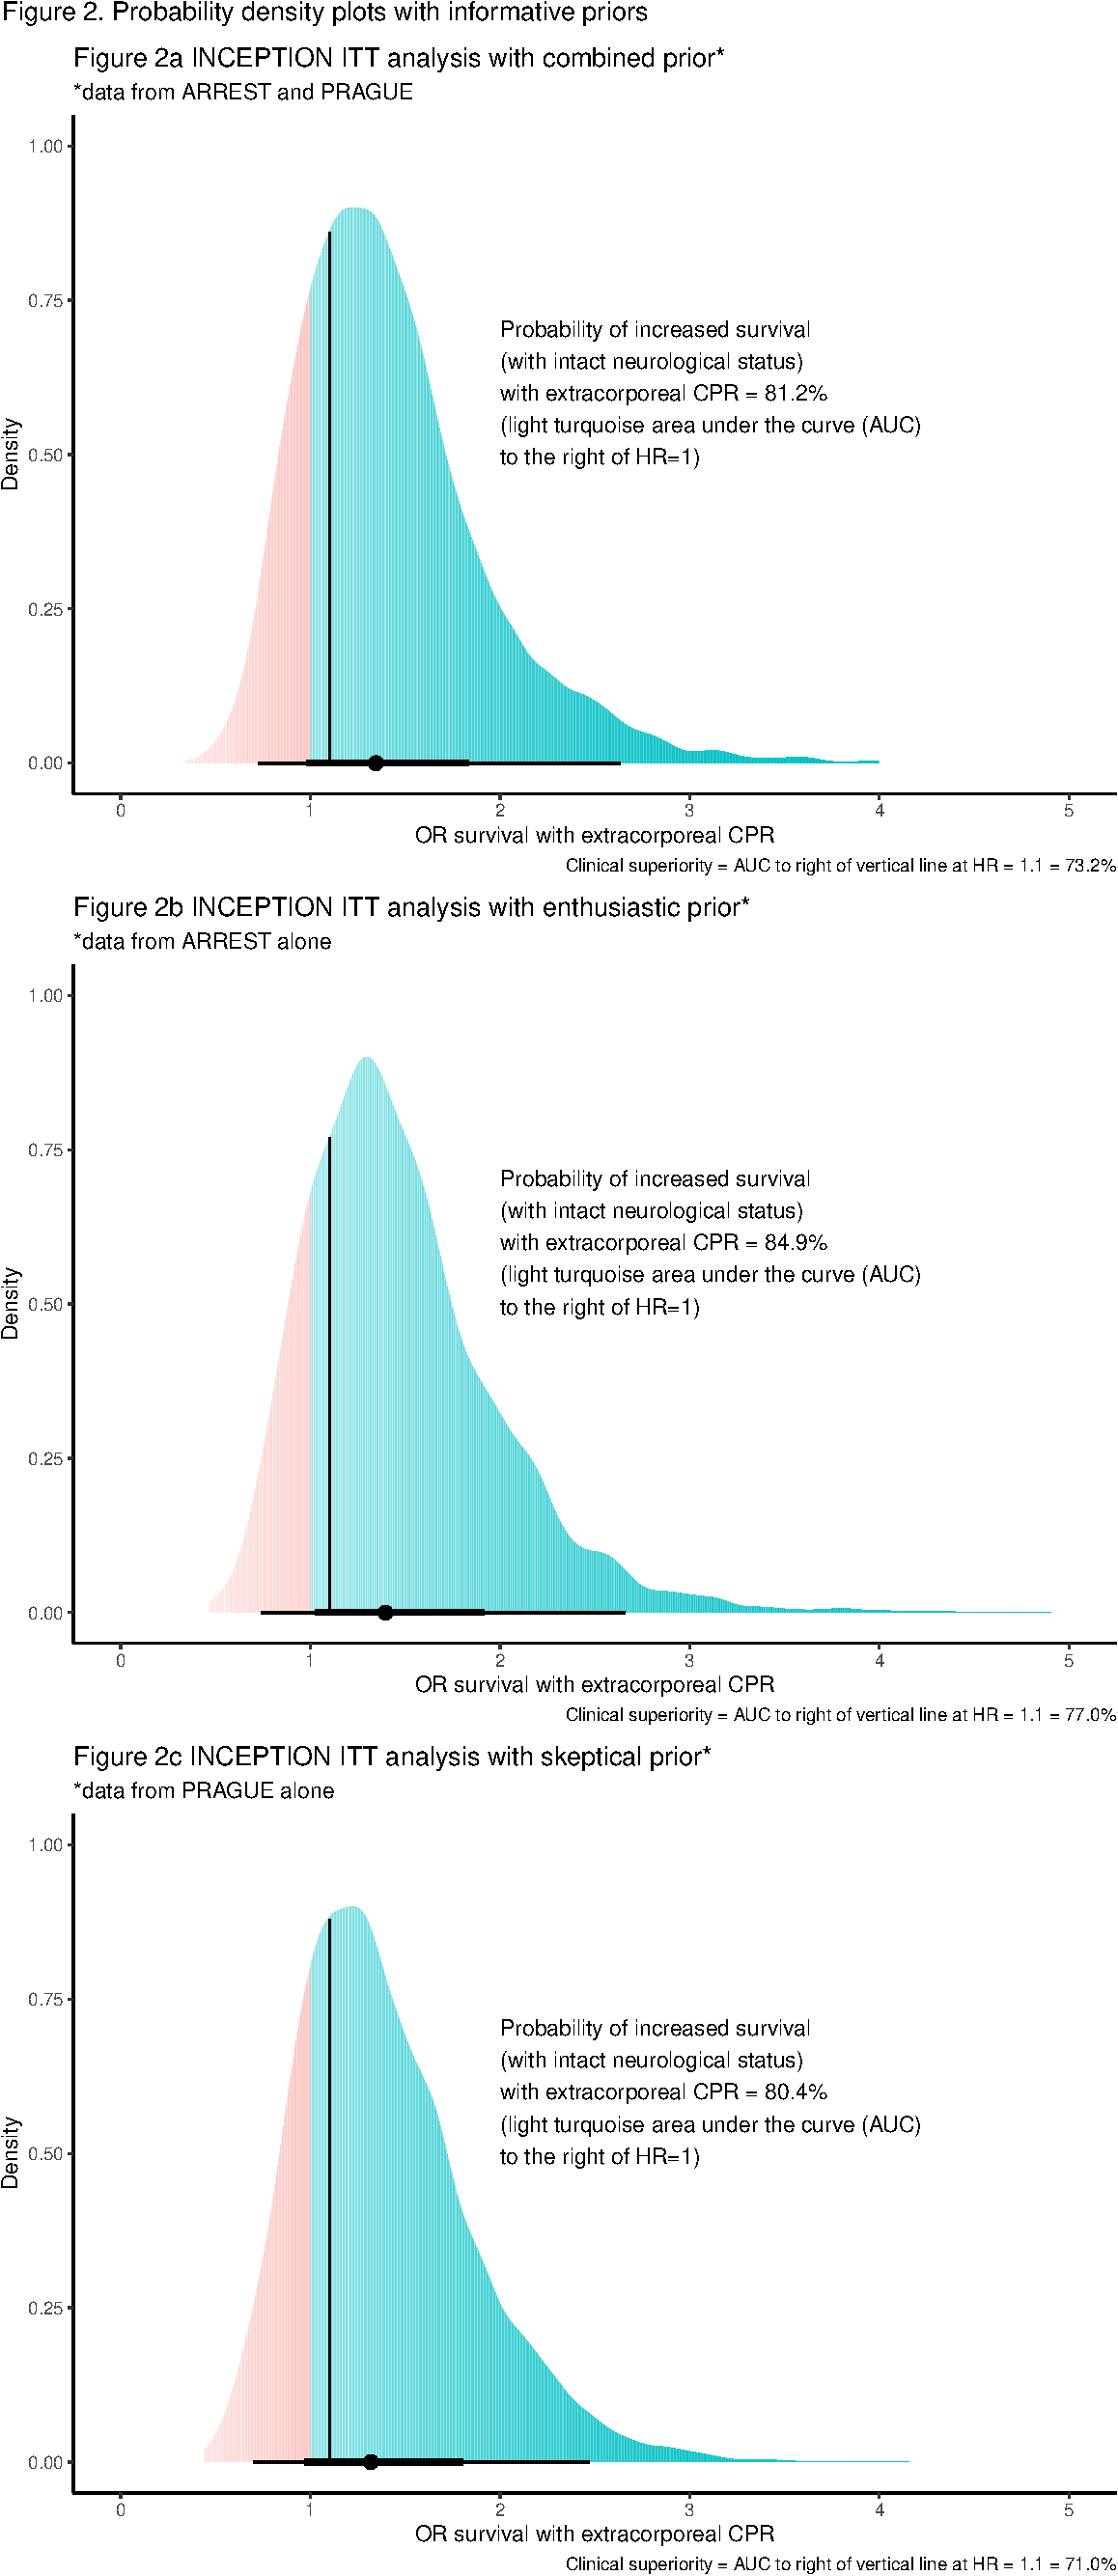
\includegraphics{manuscript_files/figure-pdf/fig2-1.pdf}

\newpage


\renewcommand\refname{References}
  \bibliography{bibliography.bib}


\end{document}
